\documentclass[12pt]{article}
\usepackage{latexblog}

% ============================================================
% Blog Metadata
% ============================================================
\blogtitle{Java GC小结}
\blogdate{2019-03-03}
\blogtags{Comment, 刨根问底, 探索分析}
\bloglang{zh}
\blogsummary{}

\begin{document}
\makeblogtitle

\begin{figure}
\centering
\pandocbounded{\includegraphics[keepaspectratio,alt={HotSpot JVM architecture}]{https://www.oracle.com/webfolder/technetwork/tutorials/obe/java/gc01/images/gcslides/Slide1.png}}
\caption{HotSpot JVM architecture}
\end{figure}

\section{JVM Generations}\label{jvm-generations}

\begin{figure}
\centering
\pandocbounded{\includegraphics[keepaspectratio,alt={Hotspot Heap Structure}]{https://www.oracle.com/webfolder/technetwork/tutorials/obe/java/gc01/images/gcslides/Slide5.png}}
\caption{Hotspot Heap Structure}
\end{figure}

Java的堆被划分成不同的区域：

\begin{itemize}
\tightlist
\item
  young generation：存放新创建的对象，当这个区域占满的时候，会触发minor GC，这时候存活的对象会被标记年龄，最终会移动到old generation。
\item
  old generation：存放存活的比较久的对象。当yound generation存活的对象年龄到达设置的阈值后，就会被移动到这里来。当这个区域满了的时候，会触发major GC。
\item
  permanent generation：存放一些JVM运行所需的元数据，例如类的信息等。full GC的时候也包括对这个区域的GC。 其中，minor GC和major GC都是Stop the World的，即当GC触发的时候，所有的程序线程都会停止等待GC完成。通常minor GC会比major GC快很多，因为major GC会遍历所有的存活对象。
\end{itemize}

其中，yound generation 又被划分成Eden space, Survivor Space1, Survivor Space2，其中Eden Space占了绝大部分的空间。当Eden space满的时候，GC 会将存活对象移动到其中一个Survivor Space中，两个Survivor Space是为了避免内存碎片，每次将存活的对象（Eden Space以及上一个Survivor Space）移动到另一个Survivor Space中。

\begin{figure}
\centering
\pandocbounded{\includegraphics[keepaspectratio,alt={Mnior GC}]{https://www.oracle.com/webfolder/technetwork/tutorials/obe/java/gc01/images/gcslides/Slide9.png}}
\caption{Mnior GC}
\end{figure}

通过Java VisualVM和VisualGC插件可以很直观的看到GC的过程: \pandocbounded{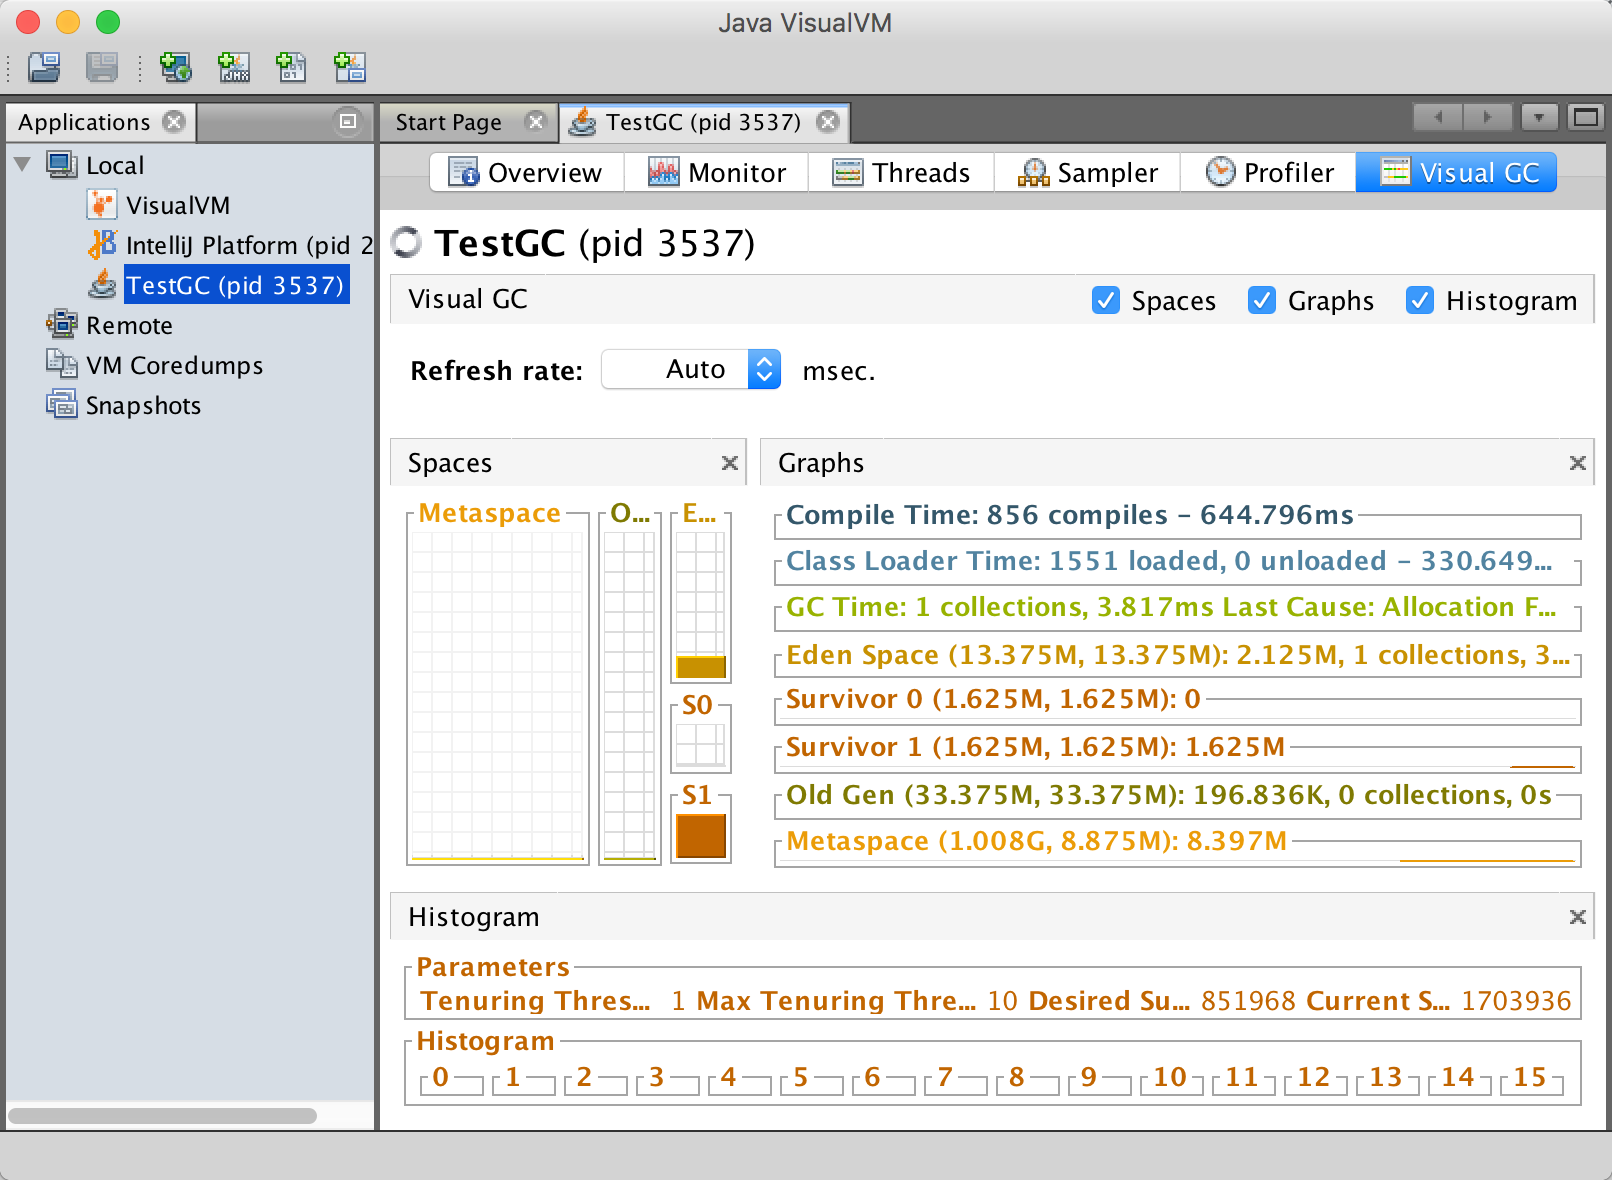
\includegraphics[keepaspectratio,alt={Visual GC}]{images/visualVM_GC.png}}

\begin{Shaded}
\begin{Highlighting}[]
\ExtensionTok{java} \AttributeTok{{-}Xmx50m} \DataTypeTok{\textbackslash{}}
\NormalTok{{-}XX:{-}PrintGC }\DataTypeTok{\textbackslash{}}
\NormalTok{{-}XX:+PrintHeapAtGC }\DataTypeTok{\textbackslash{}}
\NormalTok{{-}XX:MaxTenuringThreshold=10 }\DataTypeTok{\textbackslash{}}
\NormalTok{{-}XX:+UseConcMarkSweepGC }\DataTypeTok{\textbackslash{}}
\NormalTok{{-}XX:+UseParNewGC TestGC}
\end{Highlighting}
\end{Shaded}

\section{Garbage Collectors}\label{garbage-collectors}

{\def\LTcaptype{none} % do not increment counter
\begin{longtable}[]{@{}ll@{}}
\toprule\noalign{}
Argument & Description \\
\midrule\noalign{}
\endhead
\bottomrule\noalign{}
\endlastfoot
-Xms & Sets the initial heap size for when the JVM starts. \\
-Xmx & Sets the maximum heap size. \\
-Xmn & Sets the size of the Young Generation. \\
-XX:PermSize & Sets the starting size of the Permanent Generation. \\
-XX:MaxPermSize & Sets the maximum size of the Permanent Generation \\
\end{longtable}
}

\begin{itemize}
\tightlist
\item
  \textbf{Serial GC}:使用mark-compact算法进行GC，单线程的进行GC，适合单核CPU和在客户端允许的Java程序。
\item
  \textbf{Parallel GC(throughput collector)}:多线程进行GC
\item
  \textbf{Concurrent Mark Sweep (CMS) Collector}: 在程序运行的时候并发的进行GC，以最大限度减少停止时间
\item
  \textbf{G1(Garbage-First) Garbage Collector}: CMS的替代品
\end{itemize}

其中存在并行(Parallel)和并发(Concurrent)的区别，并行是指垃圾收集器多个线程同时工作，但此时用户线程依然是停止等待的；而并发是指在用户线程工作的同时，垃圾收集器同时执行。

\begin{figure}
\centering
\pandocbounded{\includegraphics[keepaspectratio,alt={Java collectors}]{https://cdn.app.compendium.com/uploads/user/e7c690e8-6ff9-102a-ac6d-e4aebca50425/f4a5b21d-66fa-4885-92bf-c4e81c06d916/Image/b125abbe194f5608840119eccc9d90e2/collectors.jpg}}
\caption{Java collectors}
\end{figure}

{\def\LTcaptype{none} % do not increment counter
\begin{longtable}[]{@{}llll@{}}
\toprule\noalign{}
Garbage Collector & Type & Algorithm & MultiThread \\
\midrule\noalign{}
\endhead
\bottomrule\noalign{}
\endlastfoot
Serial & stop-the-world & copying & No \\
ParNew & stop-the-world & copying & Yes \\
Parallel Scavenge & stop-the-world & copying & Yes \\
Serial Old & stop-the-world & mark-sweep-compact & No \\
CMS & low-pause & concurrent-mark-sweep & Yes \\
Parallel Old & stop-the-world & mark-sweep-compact & Yes \\
G1 & & compacting & Yes \\
\end{longtable}
}

{\def\LTcaptype{none} % do not increment counter
\begin{longtable}[]{@{}ll@{}}
\toprule\noalign{}
Arguments & Result \\
\midrule\noalign{}
\endhead
\bottomrule\noalign{}
\endlastfoot
-XX:+UseSerialGC & Serial + Serial Old \\
-XX:+UseParNewGC & ParNew + Serial Old \\
-XX:+UseConcMarkSweepGC & ParNew + CMS + Serial Old\footnote{``CMS'' is used most of the time to collect the tenured generation. ``Serial Old'' is used when a concurrent mode failure occurs.} \\
-XX:+UseParallelGC & Parallel Scavenge + Serial Old \\
-XX:+UseParallelOldGC & Parallel Scavenge + Parallel Old \\
--XX:+UseG1GC & G1 \\
\end{longtable}
}

\section{GC过程}\label{gcux8fc7ux7a0b}

\subsection{CMS}\label{cms}

CMS 收集器的步骤：

{\def\LTcaptype{none} % do not increment counter
\begin{longtable}[]{@{}ll@{}}
\toprule\noalign{}
Phase & Description \\
\midrule\noalign{}
\endhead
\bottomrule\noalign{}
\endlastfoot
Initial Mark (Stop-Word) & 标记老年代中的对象是否可达(reachable)，包括可以从新生代中到达的 \\
Concurrent Marking & \\
Remark (Stop-Word) & \\
Concurrent Sweep & \\
Resetting & \\
\end{longtable}
}

G1将Heap划分成一些相同大小的区块，但是没有限制不同代的大小。

\begin{figure}
\centering
\pandocbounded{\includegraphics[keepaspectratio,alt={G1 Heap Allocation}]{https://www.oracle.com/webfolder/technetwork/tutorials/obe/java/G1GettingStarted/images/slide9.png}}
\caption{G1 Heap Allocation}
\end{figure}

References:

\begin{itemize}
\tightlist
\item
  \href{http://enos.itcollege.ee/~jpoial/allalaadimised/reading/Advanced-java.pdf}{Advanced Java}
\item
  \href{https://codeahoy.com/2017/08/06/basics-of-java-garbage-collection/}{Basics of Java Garbage Collection}
\item
  \href{https://www.novatec-gmbh.de/en/blog/g1-action-better-cms/}{G1 in Action: Is it better than the CMS?}
\item
  \href{https://www.oracle.com/webfolder/technetwork/tutorials/obe/java/gc01/index.html}{Java Garbage Collection Basics}
\item
  \href{https://www.oracle.com/webfolder/technetwork/tutorials/obe/java/G1GettingStarted/index.html}{Getting Started with the G1 Garbage Collector}
\end{itemize}


\end{document}
